\setcounter{secnumdepth}{-1} % Убираем нумерацию секций

\section{Введение}

В данной лабораторной работе рассматриваются методы анализа 
устойчивости нелинейных динамических систем с использованием 
функций Ляпунова, а также синтез стабилизирующих регуляторов 
на основе линейных матричных неравенств (LMI).

\section{1. Анализ устойчивости с использованием кандидата квадратичной функции Ляпунова}

Для каждой из следующих систем используем кандидат квадратичной 
функции Ляпунова $V(x) = x_1^2 + x_2^2$ (для скалярной системы $V(x) = x^2$).

\subsection*{Система 1}

Рассмотрим систему:
\begin{align*}
\dot{x}_1 &= -x_1 + x_1 x_2 \\
\dot{x}_2 &= -2x_2
\end{align*}

Найдем производную функции Ляпунова $V(x) = x_1^2 + x_2^2$:
\begin{align*}
\dot{V} &= 2x_1 \dot{x}_1 + 2x_2 \dot{x}_2 \\
&= 2x_1(-x_1 + x_1 x_2) + 2x_2(-2x_2) \\
&= -2x_1^2 + 2x_1^2 x_2 - 4x_2^2 \\
&= -2x_1^2 (1 - x_2) - 4x_2^2
\end{align*}

\textbf{Анализ устойчивости:}

При $x_2 < 1$: $\dot{V} < 0$. Следовательно, система асимптотически
устойчива в окрестности начала координат, но не является глобально устойчивой.

\subsection{Система 2}

Рассмотрим систему:
\begin{align*}
\dot{x}_1 &= -x_2 - x_1(1 - x_1^2 - x_2^2) \\
\dot{x}_2 &= x_1 - x_2(1 - x_1^2 - x_2^2)
\end{align*}

Найдем производную функции Ляпунова $V(x) = x_1^2 + x_2^2$:
\begin{align*}
\dot{V} &= 2x_1 \dot{x}_1 + 2x_2 \dot{x}_2 \\
&= 2x_1\left(-x_2 - x_1(1 - x_1^2 - x_2^2)\right) + 2x_2\left(x_1 - x_2(1 - x_1^2 - x_2^2)\right) \\
&= -2x_1 x_2 - 2x_1^2(1 - x_1^2 - x_2^2) + 2x_1 x_2 - 2x_2^2(1 - x_1^2 - x_2^2) \\
&= -2(x_1^2 + x_2^2)(1 - x_1^2 - x_2^2)
\end{align*}

\textbf{Анализ устойчивости:}

При $x_1^2 + x_2^2 < 1$: $\dot{V} < 0$. Следовательно, область устойчивости 
ограничена единичным кругом, поэтому система локально асимптотически устойчива, 
но не является глобально устойчивой.

\subsection{Система 3}

Рассмотрим систему:
\begin{align*}
\dot{x}_1 &= x_2(1 - x_1^2) - 2x_1 \\
\dot{x}_2 &= -(x_1 + x_2)(1 - x_1^2)
\end{align*}

Найдем производную функции Ляпунова $V(x) = x_1^2 + x_2^2$:
\begin{align*}
\dot{V} &= 2x_1\left(x_2(1 - x_1^2) - 2x_1\right) + 2x_2\left(-(x_1 + x_2)(1 - x_1^2)\right) \\
&= 2x_1 x_2(1 - x_1^2) - 4x_1^2 - 2x_1 x_2(1 - x_1^2) - 2x_2^2(1 - x_1^2) \\
&= -4x_1^2 - 2x_2^2(1 - x_1^2)
\end{align*}

\textbf{Анализ устойчивости:}

При $x_1 < 1$: $\dot{V} < 0$. Следовательно, система асимптотически
устойчива в окрестности начала координат, но не является глобально устойчивой.

\subsection*{Система 4}

Рассмотрим систему:
\begin{align*}
\dot{x}_1 &= -3x_1 - x_2 \\
\dot{x}_2 &= 2x_1 - x_2^3
\end{align*}

Найдем производную функции Ляпунова $V(x) = x_1^2 + x_2^2$:
\begin{align*}
\dot{V} &= 2x_1(-3x_1 - x_2) + 2x_2(2x_1 - x_2^3) \\
&= -6x_1^2 - 2x_1 x_2 + 4x_1 x_2 - 2x_2^4 \\
&= -6x_1^2 + 2x_1 x_2 - 2x_2^4
\end{align*}

\textbf{Анализ устойчивости:}

При $2x_1 x_2 < 6x_1^2 + 2x_2^4$: $\dot{V} < 0$.
Неравенство выполняется для любых $x_1$ и $x_1$.
Следовательно, система глобально асимптотически устойчива.

\subsection*{Система 5}

Рассмотрим скалярную систему:
\begin{align*}
\dot{x} = -\arctan(x)
\end{align*}

Найдем производную функции Ляпунова $V(x) = x^2$:
\begin{align*}
\dot{V} &= 2x \dot{x} = 2x(-\arctan(x)) = -2x\arctan(x)
\end{align*}

\textbf{Анализ устойчивости:}

Так как $\arctan(-x) = -\arctan(x)$, то $\dot{V} < 0$ везде, кроме 0. 
Следовательно, система глобально асимптотически устойчива.


\section{2. Условия асимптотической устойчивости скалярной системы}

Рассмотрим скалярную систему:
\begin{align*}
\dot{x} = ax^p + h(x)
\end{align*}
где $p$ — натуральное число, а $h(x)$ удовлетворяет условию $|h(x)| \leq k|x|^{p+1}$ в некоторой окрестности точки начала координат.

Требуется определить условия, при которых система асимптотически устойчива.

Выберем функцию Ляпунова $V=\frac{1}{2}x^2$. Возьмем производную:
\begin{align*}
\dot{V} = x\dot{x} = x(ax^p + h(x)) = ax^{p+1} + xh(x)
\end{align*}

Учитывая условие задания 
\begin{align*}
|xh(x)| \le |x| \dot k|x|^{p+1} = k|x|^{p+2}
\end{align*}

получим 
\begin{align*}
& \dot{V} = ax^{p+1} + xh(x) \le ax^{p+1} + k|x|^{p+2} \\
& |xh(x)| \leq k|x|^{p+2} \ll |ax^{p+1}| - \text{в малой окрестности начала координат}
\end{align*}

\subsection{Случай 1: $p$ — нечетное число}

При нечетном $p$ имеем $x^{p+1} \geq 0$ для всех $x$.

\begin{itemize}
\item Если $a < 0$, то $ax^{p+1} \leq 0$ для всех $x$.
Тогда $\dot{V} < 0$ $\Rightarrow$ система асимптотически устойчива.
\item Если $a > 0$, то $ax^{p+1} \geq 0$ для всех $x$.
Тогда $\dot{V} > 0$ $\Rightarrow$ система неустойчива.
\end{itemize}

\subsection{Случай 2: $p$ — четное число}

При четном $p$ имеем $x^{p+1}$ имеет тот же знак, что и $x$.

\begin{itemize}
\item Если $a < 0$, то $ax^{p+1} < 0$ при $x > 0$ и $ax^{p+1} > 0$ при $x < 0$.
Тогда $\dot{V} < 0$ при $x > 0$ и $\dot{V} > 0$ при $x < 0$ $\Rightarrow$ система неустойчива.
\item Если $a > 0$, то $ax^{p+1} > 0$ при $x > 0$ и $ax^{p+1} < 0$ при $x < 0$.
Тогда $\dot{V} > 0$ при $x > 0$ и $\dot{V} < 0$ при $x < 0$ $\Rightarrow$ система неустойчива.
\end{itemize}

\subsection{Случай 3: $a = 0$}

При $a = 0$ имеем $\dot{x} = h(x)$. Таким образом, устойчивость системы зависит от конкретного вида $h(x)$.

\subsection{Условие асимптотической устойчивости:}
\begin{itemize}
\item $|h(x)| \leq k|x|^{p+1}$ - в малой окрестности начала координат;
\item $p$ - нечетное число;
\item $a < 0$.
\end{itemize}

\section*{Задача 3. Синтез линейного регулятора через LMI}

На основе применения LMI построим линейный регулятор, стабилизирующий систему экспоненциально со степенью 2:
\begin{align*}
\dot{x}_1 &= x_2 \\
\dot{x}_2 &= 2x_1 + u
\end{align*}

\subsection*{Постановка задачи}

Требуется найти матрицу обратной связи $K$ такую, что замкнутая система $\dot{x} = (A + BK)x$ имеет экспоненциальную устойчивость степени $\alpha$=2, то есть:

\begin{equation}
\|x(t)\| \leq ce^{-\alpha t}\|x(0)\|
\end{equation}

для некоторого $c > 0$ и всех $t \geq 0$.

Матрицы системы:
\begin{align*}
A = \begin{pmatrix} 0 & 1 \\ 2 & 0 \end{pmatrix}, \quad
B = \begin{pmatrix} 0 \\ 1 \end{pmatrix}
\end{align*}

\subsection*{Анализ управляемости}

Матрица управляемости:
\begin{align*}
U = [B, AB] = \begin{pmatrix} 0 & 1 \\ 1 & 0 \end{pmatrix} \\
rank(U) = 2
\end{align*}

Ранг матрицы управляемости равен порядку систему (n=2), следовательно система полностью управляема.

Собственные значения разомкнутой системы $\lambda = \pm\sqrt{2} \approx \pm 1.414$, что означает неустойчивость.

\subsection*{Синтез регулятора}

Синтезируем регулятор, обеспечивающий заданную степень устойчивости, 
при помощи матричного неравенства Ляпунова:
\begin{align}
& PA^T + AP + 2\alpha P + Y^T B^T + BY \preceq 0 \\
& K = YP^{-1}
\end{align}

Получим матрицу регулятора:
\begin{align*}
K = \begin{pmatrix} -7.2383 & -4 \end{pmatrix} \\
\end{align*}

Определим собственные числа матрицы замкнутой системы $(A+BK)$:
\begin{align*}
\sigma(A+BK) = \begin{pmatrix}-2 + 1.1128i \\ -2 - 1.1128i \end{pmatrix}
\end{align*}

Как видно, регулятор обеспечивает требуемую степень устойчивость.

Выполним моделирование замкнутой системы и построим
графики управления $u(t)$ и вектора состояния $x(t)$ 
при начальных условиях $x(0) = \begin{pmatrix} 1 & 1 \end{pmatrix}^T$.

\begin{figure}[H]
\centering
\begin{minipage}{0.7\linewidth}
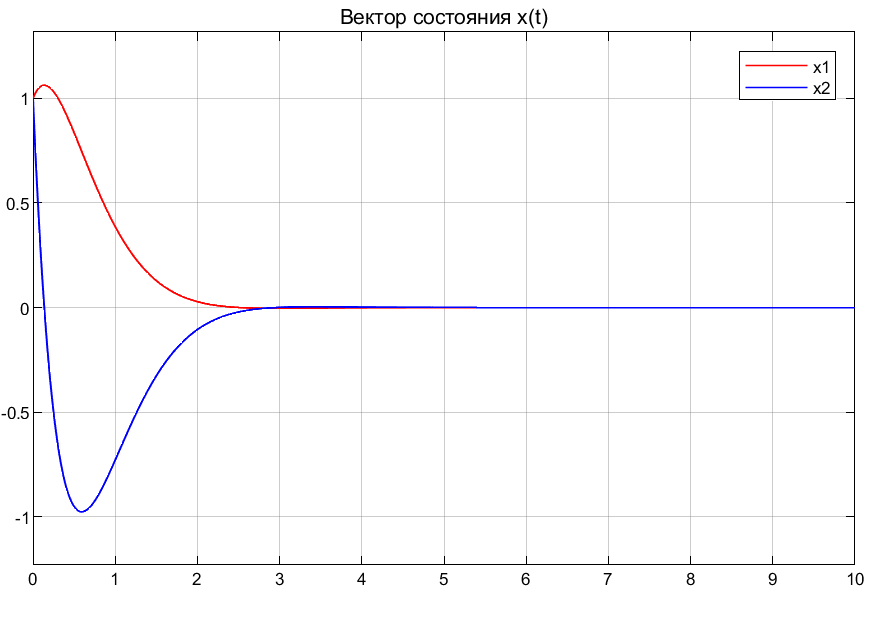
\includegraphics[width=\linewidth]{task3/state.png}
\end{minipage}
\begin{minipage}{0.7\linewidth}
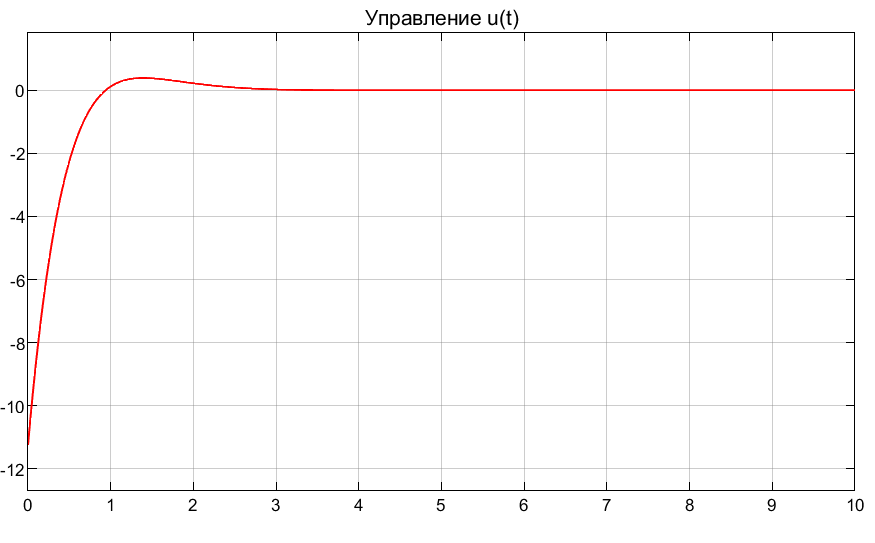
\includegraphics[width=\linewidth]{task3/control.png}
\end{minipage}
\caption{Моделирование замкнутой системы}
\label{fig:lmi_simulation}
\end{figure}

\section{Задача 4. Ограничивающее условие на параметр $\gamma$}

Найдем ограничивающее условие на параметр $\gamma$, при котором система является асимптотически устойчивой со степенью 1. Закон управления взят из предыдущего задания.

Рассмотрим систему:
\begin{align*}
\dot{x}_1 &= x_2 + \gamma \sin x_2 \\
\dot{x}_2 &= 2x_1 + u
\end{align*}

где $u = Kx$ и $K = \begin{pmatrix} -7.2383 & -4 \end{pmatrix}$ (из задачи 3).

С учетом закона управления получаем:
\begin{align*}
\dot{x}_1 &= x_2 + \gamma \sin x_2 \\
\dot{x}_2 &= 2x_1 + (-7.2383x_1 - 4x_2) = -5.2383x_1 - 4x_2
\end{align*}

Линеаризуем систему в точке равновесия $(0,0)$:
\begin{equation*}
J = \begin{pmatrix} 
\frac{\partial f_1}{\partial x_1} & \frac{\partial f_1}{\partial x_2} \\
\frac{\partial f_2}{\partial x_1} & \frac{\partial f_2}{\partial x_2}
\end{pmatrix} = \begin{pmatrix} 
0 & 1 + \gamma \cos(0) \\
-5.2383 & -4
\end{pmatrix} = \begin{pmatrix} 
0 & 1 + \gamma \\
-5.2383 & -4
\end{pmatrix}
\end{equation*}

Характеристический полином линеаризованной системы:
\begin{align*}
\det(\lambda I - J) &= \det\begin{pmatrix} \lambda & -(1+\gamma) \\ 5.2383 & \lambda+4 \end{pmatrix} \\
&= \lambda(\lambda+4) - 5.2383 \cdot (-(1+\gamma)) \\
&= \lambda^2 + 4\lambda + 5.2383(1+\gamma)
\end{align*}

Для асимптотической устойчивости степени 1 требуется, чтобы все 
собственные значения имели вещественную часть меньше $-1$.

Корни характеристического уравнения:
\begin{align*}
\lambda = \frac{-4 \pm \sqrt{16 - 20.9532(1+\gamma)}}{2} &= \frac{-4 \pm \sqrt{-4.9532-20.9532\gamma}}{2} < -1 \\
-4 \pm \sqrt{-4.9532-20.9532\gamma} &< -2 \\
\sqrt{-4.9532-20.9532\gamma} &< 2 \\
-4.9532-20.9532\gamma &< 4 \\
-20.9532\gamma &< 8.9532 \\
\gamma &< -\frac{8.9532}{20.9532} \\
\gamma &< -0.4273 \\
\end{align*}

Таким образом, при $\gamma<-0.4273$ с выбранным регулятором система является асимптотически устойчивой со степенью 1. 

\section*{Задача 5. Анализ системы с управлением u = Kx}

Рассмотрим систему:
\begin{align*}
    \begin{cases}
        \dot{x}_1 &= x_2 - 0.5x_1^3 \\
        \dot{x}_2 &= u
    \end{cases}
\end{align*}

где $u = Kx$ — линейное управление по состоянию.

1. Синтезируем линейный регулятор с обратной связью по
состоянию, чтобы глобально стабилизировать начало
координат.
Функция Ляпунова:
\begin{align*}
    V(x) = \frac{1}{2} \left( x_1^2 + x_2^2 \right)
\end{align*}

Найдем производную функции Ляпунова:
\begin{align*}
    \dot{V}(x) &= x_1 \dot{x_1} + x_2 \dot{x_2} = \\
    &= x_1(x_2 - 0.5x_1^3) + x_2(k_1x_1 + k_2x_2) = \\
    &= (1 + k_1)x_1x_2 + k_2x_2^2 - 0.5x_1^4
\end{align*}

Таким образом, глобальная асимптотическая устойчивость достигается при $k_1 = -1$ и $k_2 \le 0$.

Пусть $K = [-1 -1]$. Тогда система примет вид:
\begin{align*}
    \begin{cases}
        \dot{x}_1 = x_2 - 0.5x_1^3 \\
        \dot{x}_2 = -x_1 - x_2
    \end{cases}
\end{align*}

2. Исследуем устойчивость по входу к состоянию (ISS) при наличии
шумов измерений.

Система называется ISS, если существуют функции
$\beta \in \mathcal{KL}$ и $\gamma \in \mathcal{K}$
такие, что для любых начальных условий $x(0)$ и любого 
ограниченного входа $u(t)$ выполняется:
\begin{align*}
    \|x(t)\| \le \beta(\|x(0)\|, t) + \gamma\left(\sup_{\tau \in [0,t]} \|u(\tau)\|\right)
\end{align*}
для всех $t \ge 0$.

Пусть измерения зашумлены. Тогда
\begin{align*}
    u = K(x + \delta) = Kx + K\delta = (-x_1 - x_2) + (-\delta_1 - \delta_2)
\end{align*}

Тогда система примет вид:
\begin{align*}
    \begin{cases}
        \dot{x}_1 = x_2 - 0.5x_1^3 \\
        \dot{x}_2 = -x_1 - x_2 - \delta_1 - \delta_2
    \end{cases}
\end{align*}

Найдем производную функции Ляпунова:
\begin{align*}
    \dot{V}(x) = -0.5x_1^4 - x_2^2 - x_2(\delta_1 + \delta_2)
\end{align*}

Оценим смешанный член с помощью неравенства
\begin{align*}
    ab &\le \frac{1}{2} \left( a^2 + b_2^2 \right)\\
    -x_2(\delta_1 + \delta_2) &\le \frac{1}{2} \left(x_2^2 + (\delta_1 + \delta_2)^2 \right)
\end{align*}

Получим
\begin{align*}
    \dot{V}(x) \le -\frac{1}{2}x_1^4 - \frac{1}{2}x_2^2 + \frac{1}{2} (\delta_1 + \delta_2)^2
\end{align*}

Используя неравенство $(\delta_1+\delta_2)^2 \le 2(\delta_1^2 + \delta_2^2) = 2\|\delta\|^2$, получим
\begin{align*}
    \dot{V}(x) \le -\frac{1}{2}x_1^4 - \frac{1}{2}x_2^2 + \|\delta\|^2
\end{align*}

Следовательно, $\dot{V} < 0$ при $\frac{1}{2}x_1^4 + \frac{1}{2}x_2^2 > \|\delta\|^2$.


3. Исследуем устойчивость по входу к состоянию при наличии
аддитивных возмущений.

При наличии аддитивных возмущений система примет вид:
\begin{align*}
    \begin{cases}
        \dot{x}_1 = x_2 - 0.5x_1^3 + d_1 \\
        \dot{x}_2 = -x_1 - x_2 + d_2
    \end{cases}
\end{align*}

Найдем производную функции Ляпунова:
\begin{align*}
    \dot{V}(x) = -0.5x_1^4 - x_2^2 + x_1d_1 + x_2d_2
\end{align*}

Тогда
\begin{align*}
    \dot{V}(x) \le -0.5x_1^4 - x_2^2 + \frac{1}{2} \|x\|^2 + \frac{1}{2}\|d\|^2
\end{align*}

Следовательно, $\dot{V} < 0$ при $0.5x_1^4 + x_2^2 - \frac{1}{2} \|x\|^2 > \frac{1}{2}\|d\|^2$.

Подводя итог, при выбранном регуляторе замкнутая система 
глоабльно асимптотически устойчива без возмущений и обладает
ISS относительно шумов измерений и аддитивных возмущений.

Выполним моделирование системы без шумов и возмущений, с наличием шумов и с наличием аддитивных возмущений.

